\documentclass[12pt]{article}
\usepackage[utf8]{inputenc}
\usepackage{amsmath,amssymb,amsthm}
\usepackage{graphicx}
\usepackage{listings}
\usepackage{xcolor}
\usepackage{hyperref}
\usepackage{geometry}
\geometry{margin=1in}
\usepackage{float}

\title{Domácí úkol 08}
\author{Jáchym Kouba}
\date{\today}

% Add a dot after section numbers
\renewcommand{\thesection}{\arabic{section}.}

% MATLAB listings setup
\lstdefinestyle{mystyle}{
  language=Matlab,
  basicstyle=\ttfamily\small,
  keywordstyle=\color{blue},
  commentstyle=\color{gray},
  stringstyle=\color{teal},
  numbers=left,
  numberstyle=\tiny\color{gray},
  stepnumber=1,
  numbersep=8pt,
  tabsize=2,
  breaklines=true,
  showstringspaces=false
}
\lstset{style=mystyle}

\begin{document}
\maketitle

\newpage

\section{Příklad 1}

Mám tyto stavové matice:

\begin{equation}
\begin{aligned}
A &= \begin{bmatrix}
-0.04167 & 0 & -0.0058 \\
0.0217 & -0.24 & 0.0058 \\
0 & 100 & -2.4
\end{bmatrix} \\
B &= \begin{bmatrix}
5.2 \\
-5.2 \\
0
\end{bmatrix} \\
C &= \begin{bmatrix}
0 & 0 & 1
\end{bmatrix} \\
D &= 0.
\end{aligned}
\end{equation}

Přenos dostanu z Matlabu následovně:

\begin{verbatim}
sys = ss(A, B, C, D);
G = tf(sys)
\end{verbatim}

\begin{equation}
G(s) = \frac{-520 s - 10.38}{s^3 + 2.682 s^2 + 0.106 s + 0.01242}.
\end{equation}

Z matlabu dostanu nulu systému: $s_n = -0.02$.

Pokud označím přezkmit jako $\mathrm{OS}$ a řídicí čas jako $T_s$, tak tlumení
\(\zeta\) a vlastní frekvence \(\omega_n\) jsou:
\begin{equation}\label{eq:params}
\begin{aligned}
\zeta &= -\dfrac{\ln\bigl(\mathrm{OS}\bigr)}{\sqrt{\pi^2 + \bigl(\ln\mathrm{OS}\bigr)^2}} = 0.5912, \\[6pt]
\omega_n &= \dfrac{4}{\zeta\,T_s} = 0.0677, \\[6pt]
\end{aligned}
\end{equation}

Pomocí těchto hodnot získám charakteristický polynom
\begin{equation}
c(s) = s^2 + 0.08s + 0.004578.
\end{equation}

a jeho komplexní póly
\begin{equation}\label{eq:params}
\begin{aligned}
p_{1} &= -\zeta\,\omega_n + \mathrm{i}\,\omega_n\sqrt{1-\zeta^2} = -0.0400 + 0.0546j, \\[6pt]
p_{2} &= -\zeta\,\omega_n - \mathrm{i}\,\omega_n\sqrt{1-\zeta^2} = -0.0400 - 0.0546j.
\end{aligned}
\end{equation}

Přidám zpětnou vazbu $K = \begin{bmatrix} K_1 & K_2 & K_3 \end{bmatrix}$ a parametr pro I složku $K_I$. Dostanu nový 
systém s maticí řízení:
\begin{equation}
\begin{aligned}
A_{\mathrm{celk}} &= \begin{bmatrix} A - B\,K & B\,K_I \\
                                -C & 0 \end{bmatrix}, \\
B_{\mathrm{celk}} &= \begin{bmatrix} 0 \\
                                        0 \\
                                        0 \\
                                        1 \end{bmatrix}, \\
C_{\mathrm{celk}} &= \begin{bmatrix} C & 0 \end{bmatrix},
D_{\mathrm{celk}} = 0.
\end{aligned}
\end{equation}

Charakteristický polynom matice $A_{\mathrm{celk}}$ je:
\begin{equation}
c_{\mathrm{celk}}(s)=s^{4}+a_{3}s^{3}+a_{2}s^{2}+a_{1}s+a_{0},
\end{equation}
kde koeficienty jsou
\begin{equation}
\begin{aligned}
a_{3} &= \frac{26}{5}(K_{1}-K_{2}) + \frac{268167}{100000}, \\
a_{2} &= \frac{1716}{125}K_{1} - \frac{3145961}{250000}K_{2} - 520K_{3} + \frac{132511}{1250000}, \\
a_{1} &= \frac{1872}{625}K_{1} - \frac{77883}{312500}K_{2} - \frac{25961}{2500}K_{3} - 520K_{I} + \frac{310483}{25000000}, \\
a_{0} &= -\frac{25961}{2500}K_{I}.
\end{aligned}
\end{equation}

Polynom celkové matice je řádu 4, zatímco původní polynom je pouze řádu 2. Přidám mu tedy jeden pól, který se vykrátí 
s nulou a jeden pól hodně vlevo (např. ve vzdálenosti 100):

\begin{equation}
c_{novy}(s) = s^4 + 100.1 s^3 + 10 s^2 + 0.6177 s + 0.009143
\end{equation}

Charakteristické polynomy položím do rovnosti a dostávám výsledné koeficienty:
\begin{equation}
    K = \begin{bmatrix} -0.0042 & -18.7385 & 0.4343 \end{bmatrix}
\end{equation}
\begin{equation}
    K_I = -0.00088047
\end{equation}
Nakonec si vypíšu odezvu na jednotkový skok, která odpovídá zadání.


\begin{figure}[H]
    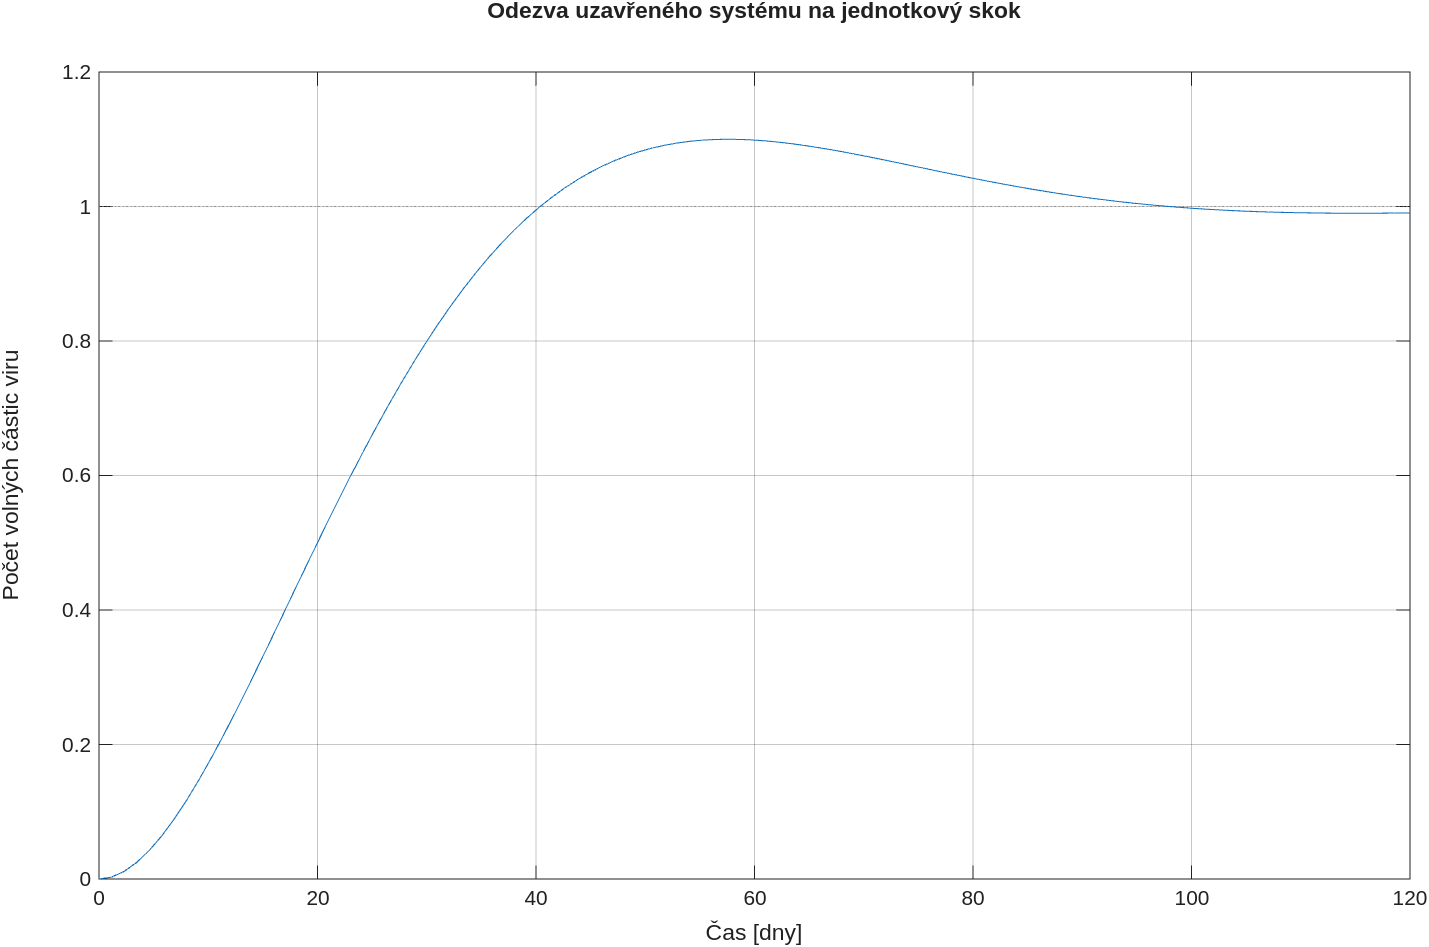
\includegraphics[width=1\textwidth]{step.png}
    \caption{jednotkový skok}
\end{figure}

\end{document}